%!TEX root = main.tex
\chapter[PRVO]{PRVO: un meta-operador para expresiones de navegaci\'on}
\label{cap:prvo}

\section{Historia de PRVO}
\label{sec:prvo.history}
En \emph{$\mu$Java} existe un operador de mutaci\'on \emph{PRV}, un operador de \textbf{P}olimorfismo para asignaciones de \textbf{R}eferencias que reemplaza la \textbf{V}ariable asignada, por otra de un tipo comparable o compatible \cite{muJavaCOPS, bibliography.mutation.operators.MaKO02}. \'Este modifica una variable que est\'a siendo asignada a una referencia (un objeto), por otra que sea compatible con la referencia, en la Figura \ref{figures.examples.PRV} vemos un ejemplo de una mutaci\'on producida por este operador. Una clara limitaci\'on de este operador es que solo aplica a asignaciones, mientras que su aplicaci\'on a otro tipo de expresiones o sentencias ser\'ia deseable. La segunda limitaci\'on est\'a precisamente en solo considerar variables, y est\'a relacionada al objetivo que tiene el operador: en lenguajes orientados a objetos, el polimorfismo permite definir m\'etodos o expresiones utilizando variables que pueden ser instanciadas por un conjunto de tipos distintos, la Figura \ref{figures.examples.polimorfism} muestra ejemplos de polimorfismo por sobrecarga y herencia, en el primer caso, para cubrir los tres m\'etodos definidos es necesario que la expresi\'on con la que se llama al m\'etodo \emph{foo} sea de tres tipos distintos, esto solo es posible con \emph{PRV} cuando se utiliza la verificaci\'on de el tipo de una instancia para cambiar el comportamiento del c\'odigo, en la Figura \ref{figures.examples.polimorfismPRV} se muestra un ejemplo del tipo de c\'odigo para el que est\'a dise\~nado este operador. Para los casos de sobrecarga mostrados en la Figura \ref{figures.examples.polimorfism}, si antes de la llamada al m\'etodo se tiene una asignaci\'on \textbf{Object o = v;}, cambiar la variable por otra, como lo har\'ia este operador, no causar\'ia que se llame a otro m\'etodo m\'as que a \emph{foo} que toma un \emph{Object}. Sin embargo modificando la variable con la que se est\'a llamando al m\'etodo si causar\'ia, dependiendo del tipo de la variable, la llamada a otra definici\'on del m\'etodo. 

\begin{figure}
	\begin{lstlisting}[mathescape=true, language=Java, extendedchars=true]
  List l = null;
  LinkedList ll = new LinkedList();
  ArrayList al = new ArrayList();
  l = ll;
  $\delta$ l = al;
	\end{lstlisting}
	\caption{Un ejemplo de una mutaci\'on de \emph{PRV} donde se reemplaza \emph{ll} por \emph{al} en la asignaci\'on original a \emph{l}}
	\label{figures.examples.PRV}
\end{figure}

\begin{figure}
	\begin{lstlisting}[mathescape=true, language=Java, extendedchars=true]
  //(i) : polimorfismo por sobrecarga
  public void foo(Integer i) {...}
  public void foo(String s) {...}
  public void foo(Object o) {...}
  ...
  foo("Test");
  foo(1);
  foo(new LinkedList());
  
  //(ii) : polimorfismo por herencia
  public void append(List a, List b) {
    for (Object o : b) {
      a.add(o);
    }
  }
  
	\end{lstlisting}
	\caption{Ejemplos de polimorfismo por sobrecarga (\emph{i}) y por herencia (\emph{ii})}
	\label{figures.examples.polimorfism}
\end{figure}

\begin{figure}
	\begin{lstlisting}[mathescape=true, language=Java, extendedchars=true,tabsize=3]
	public Number abs(Number a) {
		if (a instanceof Integer) {
			Integer res = (Integer) a;
			return -res;
		} else if (a instanceof Float) {
			Float res = (Float) a;
			return -res;
		}
		...
	}
	\end{lstlisting}
	\caption{Ejemplo de polimorfismo al cual \emph{PRV} apunta}
	\label{figures.examples.polimorfismPRV}
\end{figure}

Nuestro operador, \emph{PRVO}, surge como una extensi\'on a \emph{PRV}. No solo incluyendo las mutaciones generadas por el operador original, ahora aplicadas en cualquier contexto y no solo en la parte derecha de asignaciones, sino tambi\'en la mutaci\'on de expresiones de navegaci\'on.


\section{Expresiones de navegaci\'on}
\label{sec:prvo.navigationalExpressions}

Para definir a nuestro operador, primero necesitamos definir que consideramos a una \emph{expresi\'on de navegaci\'on}. En lenguajes orientados a objetos, el acceso a miembros de una clase es de uso com\'un, y se realiza mediante un operador de navegaci\'on que puede tomar distintas formas sint\'acticas, con la notaci\'on \emph{punto} siendo la m\'as com\'un. \'Este permite encadenar expresiones, donde la expresi\'on encadenada comienza por un miembro de la \'ultima parte expresi\'on anterior. Nos referiremos a una expresi\'on de navegaci\'on, a una que cuenta con uno o m\'as de estos operadores. El tama\~no de una expresi\'on de navegaci\'on se puede definir de distintas formas, nosotros la definiremos por el n\'umero de operadores de navegaci\'on involucrados. Una expresi\'on de navegaci\'on de tama\~no 1 entonces tendr\'ia la forma \emph{a.b}. Ejemplos de distintas expresiones de navegaci\'on se pueden ver en la Figura \ref{figures.examples.chainedExpr}, donde vale la aclarar que una vez que una expresi\'on de navegaci\'on se reduce a menos de una utilizaci\'on del operador de navegaci\'on, \'esta se considera de tama\~no 0 y ya no se considera de navegaci\'on.

\begin{figure}
	\begin{lstlisting}[mathescape=true, language=Java, extendedchars=true]
current //expresi$\'o$n de tama$\~n$o 0
null 	//expresi$\'o$n de tama$\~n$o 0
current.next //expresi$\'o$n de navegaci$\'o$n de tama$\~n$o 1
current.next.value //expresi$\'o$n de navegaci$\'o$n de tama$\~n$o 2
	\end{lstlisting}
	\caption{Ejemplos de expresiones de navegaci\'on}
	\label{figures.examples.chainedExpr}
\end{figure}

En una expresi\'on de navegaci\'on, el tipo de la misma est\'a dado por la \'ultima expresi\'on en la cadena. Por ejemplo \lstinline|a.b.c| es una expresi\'on encadenada de tama\~no dos, cuyo tipo est\'a dado por el de \emph{c}. Una expresi\'on de navegaci\'on bien tipada se puede definir de dos formas. Por pertenencia, para toda cadena \texttt{a.b}, \texttt{b} es un miembro de la clase de \texttt{a}. O mediante grafos, si cada tipo representa un nodo, y los miembros de una clase se representan como una arista que une al nodo desde el cual el miembro es alcanzable, con el nodo que representa al tipo alcanzado (no necesariamente distintos), entonces es posible generar un grafo con las posibles expresiones encadenadas v\'alidas siendo representadas por caminos dentro del grafo. Por ejemplo, la expresi\'on \lstinline|header.next.value.toString()|, es una expresi\'on de navegaci\'on de tama\~no 3, modelada mediante el grafo de la Figura \ref{figures.examples.navegationExprGraph}.

\begin{figure}
	\begin{center}
		\usetikzlibrary{positioning}
		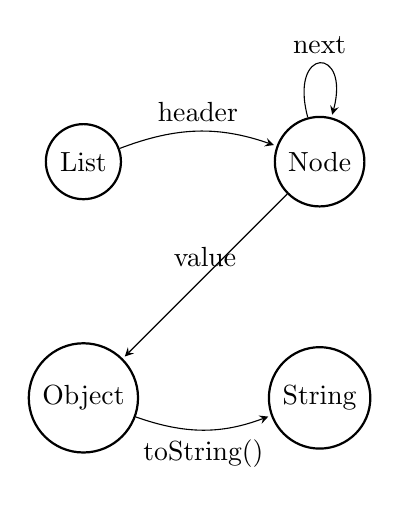
\begin{tikzpicture}%
		[>=stealth,
		shorten >=1pt,
		node distance=3cm,
		on grid,
		auto,
		every state/.style={draw=black!60, fill=black!5, very thick}
		]
		\tikzstyle{v}=[circle, minimum size=1mm,draw,thick]
		\node[v] (List)                     {List};
		\node[v] (Node) [right=of List]     {Node};
		\node[v] (Object) [below=of List]   {Object};
		\node[v] (String) [right=of Object] {String};
		
		\path[->]
		%   FROM  BEND/LOOP  POSITION OF LABEL   LABEL   TO
		(List) edge[bend left=20]     node[above] {header} (Node)
		(Node) edge[loop above]     node[above] {next} (Node)
		(Node) edge     node[above] {value} (Object)
		(Object) edge[bend right=20]     node[below] {toString()} (String)
		;
		\end{tikzpicture}
	\end{center}
	\caption{Una expresi\'on de navegaci\'on modelada mediante un grafo}
	\label{figures.examples.navegationExprGraph}
\end{figure}

\section{PRVO}
\label{sec:prvo.prvo}

Como mencionamos anteriormente, nuestro operador extiende a \emph{PRV}, \'esto lo hace de dos formas: por un lado extiende el reemplazo de variables en asignaciones a expresiones en general y extendiendo en que tipo de contextos \'estas son reemplazadas. Por el otro lado, a\~nade la modificaci\'on de expresiones de navegaci\'on. Para poder unir ambas extensiones necesitamos considerar el tama\~no de una expresi\'on como la cantidad de operadores de navegaci\'on que posee, destacando que una expresi\'on de tama\~no 0 no es considerada de navegaci\'on pero es posible convertirla en una si tiene miembros accesibles. Comenzaremos dando una descripci\'on general de \emph{prvo}:

%Todas las mutaciones que van a ser generadas est\'an centradas en expresiones encadenadas, que como definimos anteriormente, son aquellas expresiones que involucran cero o m\'as operadores de navegaci\'on, el punto en el caso de \emph{Java}. Esto significa que mutar una variable por otra es una posible mutaci\'on. En \emph{$\mu$Java}, un operador as\'i ya existe, llamado \emph{PRV} \cite{bibliography.mutation.operators.MaKO02}. En \emph{$\mu$Java++} este operador est\'a incluido en el nuestro. Teniendo en cuenta que \'este, ya es capaz de generar una cantidad significativa de mutaciones, y que pretendemos agregar mutaciones a mayor cantidad de expresiones, nos lleva a la necesidad de definir un ciertas restricciones. De todas formas, es posible dar una definici\'on general de \emph{prvo} de la siguiente manera:
\begin{quote}
	Dada una expresi\'on $e$, \emph{prvo} va a generar mutaciones al reemplazar sub-expresiones en $e$ (incluyendo a la misma $e$), respetando el tipo de la expresi\'on, y manteniendo, incrementando, o decrementando su tama\~no.
\end{quote}
La Figura \ref{figures.definitions.prvo.simple_def} da una definici\'on libre, es decir, sin ning\'un tipo de restricciones, de \emph{prvo} como una gram\'atica. Como un ejemplo simple de mutaciones de \emph{prvo}, consideremos la expresi\'on \texttt{front}, las mutaciones generadas incluyen \texttt{front.next}, \texttt{null}, \texttt{front.next.next}, \texttt{front.next.elem}, \texttt{front.next.next.next}, entre otras. Un claro problema con la definici\'on anterior es que lleva a un n\'umero potencialmente infinito de mutaciones, al no haber restricciones, como un l\'imite sobre cuanto puede incrementarse o decrementarse el tama\~no de una expresi\'on.

\subsubsection{Por que damos una definici\'on de nuestro operador que no puede usarse en la pr\'actica?}
Inicialmente parece innecesario tener una definici\'on de un operador que resulta imposible de aplicar en la pr\'actica. Pero la raz\'on detr\'as de esto es \emph{flexibilidad}. Al contrario de lo que pasa con otros operadores de mutaci\'on que suelen tener una definici\'on muy simple, como cambiar un operador por otros en un conjunto fin\'ito y predefinido, mutar expresiones tal como lo hace \emph{PRV} y como lo hace nuestra extensi\'on (que incluye a\'un m\'as expresiones a mutar) es altamente afectado por el contexto. Solo considerando \emph{PRV}, un c\'odigo donde hay una asignaci\'on a una referencia con una variable va a generar una cantidad de mutantes directamente proporcional a cuantas variables alcanzables existan y sean compatibles con la referencia en la asignaci\'on. Dado que nuestro operador extiende a \emph{PRV} tanto en que tipo de expresiones modifica, en donde y como, el contexto afecta a\'un m\'as a cuantos mutantes son generados. Determinar que expresiones utilizar al generar mutantes es algo que si bien puede automatizarse hasta cierto punto (considerando por ejemplo la clase que se est\'a mutando) sigue siendo un problema que va a ser mejor resuelto por la persona que est\'a realizando el an\'alisis y tiene conocimiento de cuales son las expresiones m\'as significativas, de la misma forma que el elegir que operadores se utilizan queda a cargo de quien hace el an\'alisis. Adem\'as, el objetivo a lograr con nuestro operador puede cambiar, con respecto a que tipo de fallas se quiere representar. De \'esta forma, dar una definici\'on inicialmente acotada nos restringe demasiado que fallas podemos representar y como.

\begin{figure}
	\begin{displaymath}
	\begin{array}{lll}
	PRVO(x)		& :=	& expression \\
	& := & PRVO(x).expression \\
	& := & expression.PRVO(x) \\
	\\
	PRVO(x.y)	& :=	& expression^{*} \\
	& :=	& PRVO(x).expression \\
	& :=	& expression.PRVO(y) \\
	& :=	& PRVO(x).expression.PRVO(y) \\
	& :=	& expression.PRVO(x).PRVO(y) \\
	& :=	& PRVO(x).PRVO(y).expression \\
	\\
	
	\multicolumn{3}{l}{\tiny{^{*} \: : \: puede \: incluir \: x \: or \: y}} \\
	\multicolumn{3}{l}{\tiny{expresi\'on \: : \: llamada \: a \: m\'etodo \: , \: acceso \: a \: atributo \: , variable \: \'o \: literal}}
	\end{array}
	\end{displaymath}
	\caption{Definici\'on abstracta de \emph{prvo}}
	\label{figures.definitions.prvo.simple_def}
\end{figure}

\subsubsection{Por qu\'e decimos que prvo es un ``meta-operador''?}
En general, un operador de mutaci\'on se define como una serie de reglas del estilo ``a partir de X genera Y'', y su uso se decide en base a sus pros y cons. En el caso de \emph{prvo}, contamos con una definici\'on que en principio no es pr\'actica, generar un n\'umero potencialmente infinito de mutaciones evidentemente nos impide su uso, limitar el cambio de tama\~no en las expresiones generadas es totalmente posible, pero cada l\'imite podr\'ia ser correctamente argumentado. A su vez, incluso limitando el tama\~no, existen muchos factores a considerar, como propiedades de las expresiones a mutar, por ejemplo solo mutar expresiones de navegaci\'on y que se encuentren en la parte derecha de sentencias de asignaci\'on. Claramente, al usar \emph{prvo}, va a ser necesario contar con estas limitaciones, pero cuales van a ser depender\'an del caso particular. Es por \'esto que consideramos \emph{prvo} como un meta-operador, en el sentido que define una potencial familia de operadores donde cada uno es una configuraci\'on particular.

%La definci\'on general de \emph{prvo} es muy similar a la de un generador de sentencias que pertenecen a una gram\'atica. Donde los t\'ipos definen a la misma. Si hubiera un programa definido mediante expresiones encadenadas y tipos, en donde encontrar\'iamos expresiones como \lstinline|if(a.gt().b).then(result.assign(a)).else(result.assign(b)).return(result)|, \emph{prvo} podr\'ia generar cualquier programa correcto desde un punto de vista de tipos. Principalmente por que las expresiones que puede utilizar no est\'an restringidas en absoluto. Esta caracter\'istica hace que \emph{prvo} sea completamente inservible para mutation testing. Lo que obliga a establecer restricciones, esto sin embargo, es una caracter\'istica positiva de \emph{prvo}, ya que cualquier operador en la familia de operadores \emph{prvo}, es en realidad una configuraci\'on particular de la misma. Lo que nos permite definir operadores a medida y aumentar la eficiencia de los mismos para cada caso.

Teniendo en cuenta los criterios para el dise\~no de operadores de mutaci\'on, discutidos en \ref{sec:preliminares.mutation.opevaluation}, en particular con respecto al n\'umero de mutaciones que un operador produce, es necesario proveer algunas cotas razonables para la aplicaci\'on de \emph{prvo}. El n\'umero de mutantes generados por \emph{prvo} puede ser limitado al limitar tres caracter\'isticas: las expresiones \emph{objetivo} (donde se va a aplicar \emph{prvo}); el \emph{tama\~no de las expresiones}, por cuanto se permite cambiar, incrementar o reducir, el tama\~no de las expresiones resultantes (las mutaciones); y los \emph{reemplazos}, es decir, las expresiones que se van a usar para el intercalado/substituci\'on en \emph{prvo}. En cuanto a los objetivos, \emph{prvo} solo va a ser aplicado a expresiones de navegaci\'on, es decir, expresiones que involucran al menos una navegaci\'on. Respecto al tama\~no, vamos a limitar \emph{prvo} a producir expresiones del \emph{mismo} tama\~no que la expresi\'on original (el n\'umero de navegaciones se mantiene). En cuanto a los reemplazos, solo vamos a reemplazar expresiones con otras de exactamente el mismo tipo (al contrario de considerar definiciones menos estrictas, que permitir\'ian utilizar tipos compatibles m\'as generales), que pertenezcan a la misma clase en donde se encuentra la expresi\'on original, o en clases directamente alcanzables desde esta clase.

Hemos definido un operador de \emph{prvo} como una serie de restricciones a la definici\'on abstracta/general. Esto nos permite centrarnos en cierto tipo de fallas particulares sin perder la habilidad de eventualmente generar otra configuraci\'on que se centra en otras.

\section{Fallas asociadas a PRVO}
\label{sec:prvo.prvoTargetedFaults}

En \cite{bibliography.mutation.evaluation.valid-substitute} se concluye que cierto tipo de fallas reales requieren mejorar operadores existentes o definir nuevos operadores de mutaci\'on para representarlas. Mientras que cierto tipo de fallas reales se consideran como imposibles de acoplar a mutantes. En esta tesis estamos interesados en aquellas fallas que pueden ser acopladas a \emph{prvo}, aun cuando algunas de estas solo puedan ser parcialmente acopladas, en referencia a que solo un subconjunto de las mismas pueden representarse mediante \emph{prvo}. En cuanto a las fallas que nos interesan, es necesario especificarlas de la forma m\'as completa posible, y analizar como deber\'iamos configurar un ``operador'' en \emph{prvo}, como mencionamos anteriormente, cada \emph{operador} no se asocia directamente con un conjunto de funciones como ocurre en la pr\'actica, sino que se refiere a una serie de restricciones particulares sobre funciones fijas ya definidas.

\subsection{Fallas que requieren mejorar operadores existentes}

\subsubsection{Eliminaci\'on de sentencias}

Una sentencia olvidada, donde un ejemplo simple es la implementaci\'on de un ciclo infinito con una sentencia de retorno bajo cierta condici\'on (Figura \ref{figures.examples.infCicle}); una sentencia \emph{switch} en donde para alg\'un caso no se escribi\'o una sentencia de retorno o frenado (\emph{break}); inicializaciones faltantes como en la Figura \ref{figures.examples.localVariableHidingField} donde una variable local utiliza el mismo nombre que un campo de clase, la falta de la sentencia que define esta variable resulta en un programa que compila pero incorrecto. \'Estos, entre otros casos, son todos ejemplos de fallas reales que requieren un operador que elimine sentencias para poder generar el mismo tipo de falla.

\begin{figure}
	\begin{lstlisting}[frame=single, mathescape=true,framexleftmargin=1.5em]
  while(true) {
    String input = getUserInput();
    if (isExitCommand(input)) {
      break;
    }
    ...
  }
	\end{lstlisting}
	\caption{Ejemplo de un ciclo infinito con una sentencia \emph{break} asociada a una condici\'on particular}
	\label{figures.examples.infCicle}
\end{figure}

\begin{figure}
	\begin{lstlisting}[frame=single, numbers=left, mathescape=true,framexleftmargin=1.5em]
  private Node cursor ...
	
  public boolean find(int elem) {
    Node cursor = header;
    while(cursor != null) {
      if (cursor.elem == elem) return true;
      cursor = cursor.next;
    }
    return false;
  }
	\end{lstlisting}
	\caption{Ejemplo en donde una inicializaci\'on faltante (linea 3), producir\'ia un programa que compila pero incorrecto}
	\label{figures.examples.localVariableHidingField}
\end{figure}

En principio, ya existen operadores que realizan este tipo de mutaciones. No solo eso, sino que adem\'as no parece ser un tipo de fallas asociadas a mutaciones de expresiones de navegaci\'on.

\begin{figure}
	\begin{lstlisting}[frame=single, mathescape=true,framexleftmargin=1.5em]
  list.foreach().filter(c1).if(c2).then(p1).else(p2)
	\end{lstlisting}
	\caption{Versi\'on utilizando \emph{interfaces fluentes} del recorrido de una lista filtrando y ejecutando condicionalmente un procedimiento.}
	\label{figures.examples.fluent.example1.fluent}
\end{figure}

Sin embargo, \emph{Fluent interfaces}, un dise\~no muy usado en conjunto con el \emph{patr\'on Builder}, permite escribir algoritmos sem\'anticamente equivalentes a un programa imperativo, ciclos y sentencias condicionales inclu\'idas. Un c\'odigo como el mostrado en la Figura \ref{figures.examples.fluent.example1.fluent} no es extra\~no en programaci\'on orientada a objetos, en la Figura \ref{figures.examples.fluent.example1.imperative} se muestra la implementaci\'on m\'as com\'un de esta expresi\'on en lenguaje imperativo.

\begin{figure}
	\begin{lstlisting}[frame=single, mathescape=true,framexleftmargin=1.5em]
  List<Elem> list = ...;
  for (Elem e : list) {
    if (c1(e)) {
      if (c2(e)) {
        p1(e);
      } else {
        p2(e);
      }
    }
  }
	\end{lstlisting}
	\caption{Versi\'on en lenguaje imperativo del recorrido de una lista filtrando y ejecutando condicionalmente un procedimiento.}
	\label{figures.examples.fluent.example1.imperative}
\end{figure}

Esto muestra que por un lado es interesante poder mutar expresiones de navegaci\'on de este tipo. Adem\'as, uno de los principales problemas con operadores que eliminan o insertan sentencias, es que suelen generar numerosos mutantes triviales que son detectados por no compilar o por que se elimin\'o directamente una gran parte de c\'odigo por una sentencia de control faltante. En \emph{interfaces fluentes}, el uso de jerarqu\'ia de tipos para garantizar la correctitud de una expresi\'on garantiza que nunca va a ser posible eliminar una sentencia cuando \'esta es necesaria.

\subsubsection{Intercambio de argumentos}

Este tipo de fallas involucra utilizar argumentos con tipos correctos, pero en el orden incorrecto en la llamada a un m\'etodo. En la Figura \ref{figures.examples.argumentSwap.example1} se ve un m\'etodo que toma como entrada dos listas y agrega la primera al final de la segunda. Los nombres de los argumentos son quiz\'as amb\'ig\"{u}os, y ser\'ia incluso esperable que sin una documentaci\'on apropiada, haya programadores que asuman que se hace un \emph{append} de \texttt{thiz} \emph{en} \texttt{that}, aunque otros podr\'ian entender de que el \emph{append} se hace con el orden de los argumentos resultando en \texttt{that} \emph{en} \texttt{thiz}. 

\begin{figure}
	\begin{lstlisting}[frame=single, mathescape=true,framexleftmargin=1.5em]
  public void append(List<E> thiz, List<E> that) {
    ...
    for (E e : thiz) {
      that.append(e);
    }
  }
	\end{lstlisting}
	\caption{M\'etodo que agrega una lista al final de otra.}
	\label{figures.examples.argumentSwap.example1}
\end{figure}

Este tipo de fallas es equivalente a aplicar dos mutaciones de cambio de referencias, \lstinline|append(thiz,that) -> append(that,that) -> append(that,thiz)|. Un tipo de mutaci\'on de expresiones como las heredadas de \emph{PRV}, salvo que requiere dos cambios en una misma mutaci\'on. Este tipo de mutaciones no puede definirse como una serie de restricciones a la definici\'on de \emph{prvo} ya que incluye definiciones extra para incluir m\'ultiples cambios. Sin embargo vale la pena notar que con dos mutaciones de \emph{prvo} podr\'ia lograrse.

\subsubsection{Llamada a un m\'etodo similar de la misma librer\'ia}

Existen ejemplos de m\'etodos que si bien distintos, tienen una sem\'antica relacionada, \texttt{indexOf} y \texttt{lastIndexOf} son dos m\'etodos de la clase \emph{java.lang.String} que permiten obtener el primer o el \'ultimo \'indice de ocurrencia de una subcadena, respectivamente. Un operador que modifique una llamada a un m\'etodo por todas las posibles, generar\'ia una cantidad demasiado grande de mutantes para ser \'util. Sin embargo cometer una equivocaci\'on al usar un m\'etodo por otro con una sem\'antica similar y provisto por la misma clase o librer\'ia, es com\'un. Este es un caso de un tipo de fallas que se pueden generar utilizando restricciones sobre \emph{prvo}.

\subsection{Fallas que requieren nuevos operadores}

\subsubsection{Omitir la llamada a un m\'etodo}

Retomemos el ejemplo de \emph{interfaces fluentes} de la Figura \ref{figures.examples.fluent.example1.fluent}. Si en este c\'odigo nos olvid\'aramos de llamar \texttt{filter(c1)}, la expresi\'on seguir\'ia siendo correcta, solamente que aplicar\'iamos el tratamiento condicional a todos los elementos de la lista en lugar de solo a aquellos que filtrar\'ia \texttt{c1}. Un ejemplo m\'as sencillo, una aplicaci\'on que toma un valor dado por el usuario y realiza una consulta en una base de datos. Es un caso t\'ipico de uso de datos no confiables, lo normal es limpiar o validar los datos ingresados antes de hacer la consulta. Una posible implementaci\'on ser\'ia:
\begin{lstlisting}
...
userQuery = getFromUser();
results = database.execute(cleanQuery(query));
...
\end{lstlisting}
Un error cl\'asico ser\'ia que el desarrollador olvide de usar \texttt{cleanQuery(query)} y directamente use \texttt{query}. Ambos casos responden a configuraciones particulares de \emph{prvo}. El primer caso, restringir las expresiones objetivo a llamadas a m\'etodos, involucradas en una expresi\'on de navegaci\'on. El segundo caso responde a restringir las expresiones objetivo a llamadas a m\'etodos en casos donde \'esta ocurra en una condici\'on, argumento u asignaci\'on, siempre que el tipo de retorno del m\'etodo sea igual o compatible con el del argumento usado en la llamada. Para los ejemplos anterior se obtendr\'ian los mutantes \lstinline|list.foreach().if(c2).then(p1).else(p2)| y:
\begin{lstlisting}
...
userQuery = getFromUser();
results = database.execute(query);
...
\end{lstlisting}

\subsubsection{Acceso directo a un campo}

Un caso particular del tipo de fallas por omitir la llamada a un m\'etodo, es el acceso a campos de clase de manera directa, en lugar de mediante el m\'etodo \emph{getter} asociado. Usualmente para cualquier atributo \emph{x} de una clase al cual se desea dar acceso, se genera un m\'etodo \emph{getX()} del mismo tipo y conteniendo solo una sentencia de retorno \emph{return x}. Sin embargo, existen casos donde el m\'etodo \emph{getter} realiza mas tareas que solo retornar. Un ejemplo muy simple es un m\'etodo que retorna una colleci\'on, cuando el campo asociado es nulo, el m\'etodo se asegurar\'ia de retornar una lista vac\'ia, en este caso utilizar el m\'etodo \emph{getter} asegura que siempre vamos a obtener una colleci\'on, mientras que acceder directamente al campo, nos puede retornar un valor nulo y causar errores como \emph{NullPointerException} en Java. Un ejemplo de este tipo de fallas se muestra en la Figura \ref{figures.examples.getterVsDirectAccess}, cuando \emph{MyStructure\#intValues} es \emph{null}, el acceso directo generar\'ia una \emph{NullPointerException}.

\begin{figure}
	\begin{lstlisting}[frame=single, numbers=left, mathescape=true,framexleftmargin=1.5em]
  MyStructure s = ...;
  for (int elem : s.getIntValues()) ...
  $\Delta$for (int elem : s.intValues) ...
	\end{lstlisting}
	\caption{Acceso a campo mediante m\'etodo \emph{getter} vs acceso directo ($\Delta$).}
	\label{figures.examples.getterVsDirectAccess}
\end{figure}

\subsubsection{Conversi\'on de tipos}

Muchas veces existen conversiones no visibles de tipos num\'ericos. Una divisi\'on \texttt{2/3} no da lo mismo que \texttt{2/3.0}, aunque es dif\'icil darse cuenta durante el desarrollo de un programa. Estas situaciones involucran en general \emph{casteos} expl\'icitos de tipos, \texttt{2/(float)3}, o uso de valores que especif\'ican claramente el tipo particular, \texttt{3.0f}. Fallas de este tipo no est\'an representadas por operadores actuales, ya que en muchos casos el error, finalmente se produce por el acarreo de numerosas p\'erdidas de precisi\'on. Aunque no relacionado con expresiones de navegaci\'on, este tipo de fallas artificiales se puede definir en base a restricciones sobre \emph{prvo}, dada una expresi\'on num\'erica, las posibles mutaciones son nuevas expresiones con el mismo valor pero distinto tipo.

\subsection{Fallas no asociadas a mutantes}

Las fallas en esta categor\'ia, son aquellas que no pueden ser acopladas a operadores de mutaci\'on. Las razones que evitan esto se pueden dividir en casos donde no es posible definir un operador dado que ser\'ia necesario dar una definici\'on por cada falla particular que se quiere representar. Y aquellos casos donde si bien es posible dar una definici\'on general, como \emph{reemplazar una llamada a un m\'etodo por todas las posibles}, lleva a una cantidad intratable de mutantes. Incluso cuando estas fallas se definen como incapaces de ser acopladas a operadores de mutaci\'on, es decir, no se puede definir un operador que las represente de manera eficiente. Creemos que es posible mediante \emph{prvo} poder representar algunos subconjuntos de las mismas.

\subsubsection{Modificaci\'on o simplificaci\'on del algoritmo}

Las fallas en este conjunto son aquellas que se dan por un algoritmo incorrecto en lugar de un algoritmo defectuoso. Mutation testing parte de asumir que el programador es competente y escribe programas cercanos a la soluci\'on correcta, si esto no se cumple, y el programa difiere significativamente, tal que se dificulta encontrar una versi\'on ``cercana'' y correcta del programa, mutation testing se vuelve inaplicable. Esto no significa que no es posible construir una falla que represente estos casos, pero no es posible hacerlo de manera general, lo que imposibilita dise\~nar un operador que represente este conjunto de fallas. Pero si nos quedamos con el subconjunto de algoritmos implementados mediante \emph{interfaces fluentes}, ahora llevamos el problema a realizar cambios en una expresi\'on de navegaci\'on, y esto es precisamente lo que hace \emph{prvo}. Como mencionamos, cualquier ``operador'' \emph{prvo} es una configuraci\'on, que define restricciones sobre que expresiones se van a modificar y como, siendo las expresiones generadas, v\'alidas respecto a tipos. Si restringimos a utilizar solo expresiones pertenecientes a los tipos utilizados por una \emph{interfaz fluente}, mientras el tipo del primer elemento de la expresi\'on original, y el del \'ultimo, se mantienen fijos, entonces podemos generar ``programas'' que trabajan sobre el mismo tipo de entradas que el original, y que retornan el mismo tipo que el original, y cuan diferentes estos ``programas'' pueden ser del original, depende en gran medida de los l\'imites a cuanto se puede modificar el tama\~no de la expresi\'on original. En estos casos, modificar un algoritmo es totalmente posible, aunque es necesario controlar las restricciones impuestas para no caer en una explosi\'on de mutantes a analizar.

\subsubsection{C\'odigo no requerido} %REVISAR TITULO

Existen fallas causadas por c\'odigo que no deber\'ia estar, es decir, cuando la reparaci\'on asociada es eliminar c\'odigo, ya sea una l\'inea o varias (no necesariamente secuenciales). Por ejemplo:
\begin{lstlisting}
	...
	if (c) breakProgram();
	...
\end{lstlisting}
En donde la reparaci\'on no es una condici\'on mal escrita sino directamente la eliminaci\'on de ciertas l\'ineas de c\'odigo. Si se quisiera representar este tipo de fallas ser\'ia necesario generar c\'odigo e insertarlo, la complejidad de generar c\'odigo v\'alido y la cantidad que se puede generar, sumado a la cantidad de lugares en donde se puede insertar, hacen que este tipo de fallas no puedan ser representadas mediante mutaci\'on. Sin embargo, \'este caso, es muy similar al anterior cuando se toman en cuenta como programas, a expresiones que utilizan \emph{interfaces fluentes}.

\subsubsection{Llamada a m\'etodos similares}

Si bien el tipo de fallas en donde se utiliza un m\'etodo similar de una librer\'ia fue mencionado como acoplable a mutantes. Eliminar la restricci\'on de que los m\'etodos pertenezcan a la misma librer\'ia, causa que el espacio posible de mutantes se convierta en completamente inmanejable. Lo \'unico que vale la pena destacar de este tipo de fallas en relaci\'on a \emph{prvo}, es que es posible, mediante configuraciones, considerar un conjunto acotado de m\'etodos que no necesariamente pertenezcan a la misma librer\'ia.

\subsubsection{Violaci\'on de especificaciones}

En mutaci\'on, el conocimiento que se tiene del c\'odigo a mutar es, a lo sumo, contexto: que elementos son alcanzables en un determinado punto del c\'odigo; tipos: cual es el tipo de una variable, el retorno de un m\'etodo, los par\'ametros del mismo, etc. Pero no existe un conocimiento de que hace un determinado c\'odigo, que precondiciones requiere y que postcondiciones asegura. Representar fallas causadas por el mal uso con respecto a invariantes, precondiciones y postcondiciones, es entonces imposible de conseguir. Sin embargo, un caso particular que creemos que \emph{prvo} puede ser de gran utilidad, es en dise\~nos basados en encadenar m\'etodos (interfaces fluentes, builder pattern, entre otros). En estas situaciones el programador debe utilizar jerarqu\'ia de clases para definir una gram\'atica, donde todo m\'etodo involucrado tiene una precondici\'on y postcondici\'on basada en tipos. Con \emph{prvo} es posible generar mutantes que permitan analizar si \'estas son incumplidas.

